\section{CUDA课程项目三：向量加法（Vector Addition）讲解}

欢迎大家。在今天的文章中，我将解释我们的第三个项目——向量加法（VectorAddition）。明确一下，这是向量A，包
含1024个元素，索引范围从0到1023。在这个项目中，我假设我们有两个向量，每个向量包含1024个元素。类似地，我们有
向量B，如图所示。当前的任务是相加这两个向量，结果将存储在向量C中，如图所示。这意味着向量A的第一个元素将与向量B的第一
个元素相加。加法操作将以逐元素的方式在每个元素上进行，结果将存储在C的零位置，也就是C的第一个元素。

\subsection{CPU上的向量加法}

在我们深入GPU代码之前，我想先展示一下这个应用在CPU上的代码。在每次迭代中，我们将向量A和向量B的对应元素相加，并将
结果保存在向量C中。如图所示，这个过程简单地涉及编写一个for循环来遍历所有元素，即1024个元素。以上就是关于在CPU
上运行向量加法的全部内容。但我们需要知道，for循环的迭代将是顺序执行的，而不是并行的。

\begin{figure}
    \centering
    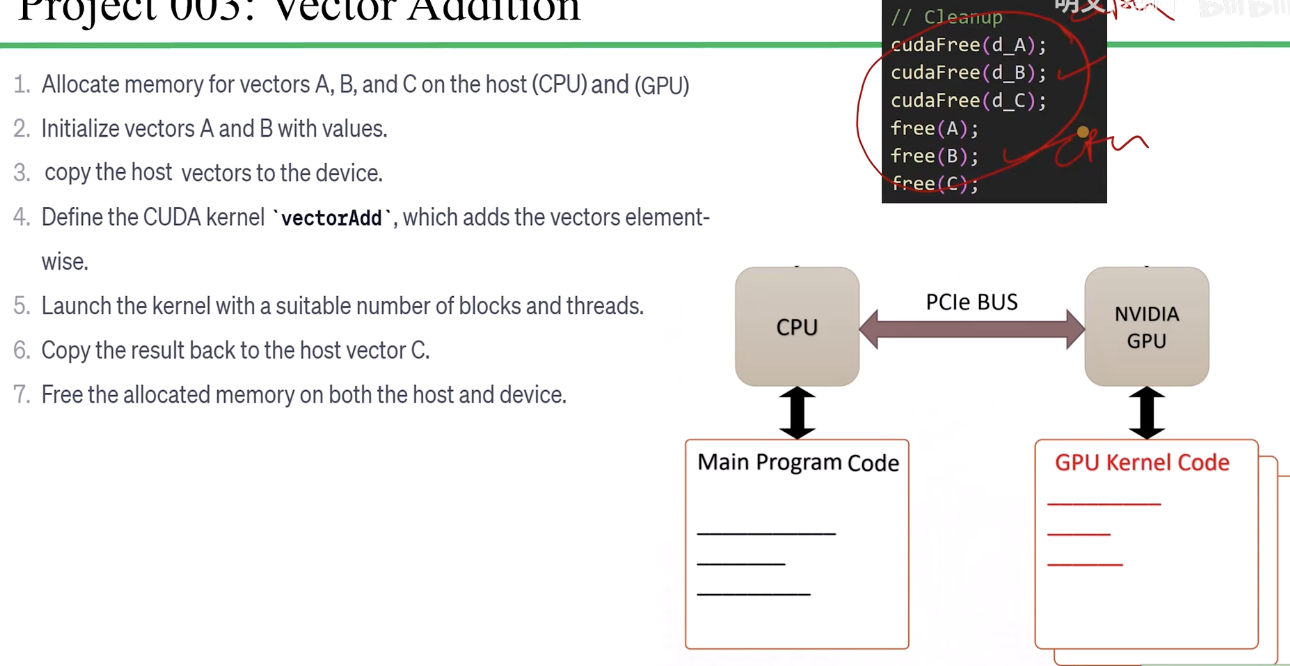
\includegraphics[width=0.75\linewidth]{resources/cuda-075.png}
    \caption{}
    \label{fig:placeholder}
\end{figure}


基于我们之前的讨论，第一步是为我们的GPU应用确定块和线程的数量。让我们探讨这个应用如何在GPU上运行。这里我首先假设只
使用一个块和1024个线程。根据这个信息，我们可以说这里的这个块它的ID将是0，而线程ID的范围将从0到1023。这个选
择使线程数量与每个向量中的元素数量一致。如果你还记得，我说过每个向量有1024个元素，这意味着每个线程ID等于向量中某个
元素的索引。我们只需要再过一分钟就需要这个信息。

很好，现在我们来写出第一个元素的加法操作，仅仅是第一个元素。一个小例子看起来是这样：C的零位置等于A的零位置加上B的零位
置，对吧？考虑到块和线程的ID，在我们的例子中只有一个块，ID是0，这完全没有用。这个模式被复制到第二个元素、第三个元素
，依此类推，覆盖了这些向量中的所有元素。我们不需要块ID，它只是一个零值。然而线程ID表明，正如我们所说，它们等于元素的
索引。这个观察使我们能够有效地为每个线程分配不同的元素。线程ID范围从0到1023，与元素的索引范围相同。例如，线程0可
以与第一个元素对齐，第二个线程可以与第二个元素对齐，以此类推。

\subsection{CUDA核函数实现}

理论部分我们已经讲完了，但现在的问题是这个理论部分如何转化为CUDA代码。实际上这个问题的答案非常简单，实现我们目标所需
的代码很简单，我们这里只需要一个操作——加法操作。这意味着我们将有一个指令或一个操作由多个线程执行。在展示的代码中，声明
了一个名为\texttt{vectorAdd}的GPU内核。然后在接下来的指令中，我们对每个元素执行加法操作。在这个内核
的第一条指令中，我们首先读取线程ID，它的范围从0到1023。因为这里的每个块以及整个GPU的线程总数等于1024。这里
的操作将被执行多次，次数等于线程数。这里的线程ID控制着将要执行加法操作的元素。这1024条指令将被分配给GPU中不同的
核心，以便并行执行。这意味着这条指令将被显式地重写1024次，每次都有一个不同的线程ID。正如这部分提到的，在GPU上相
加这两个向量的内核只需要展示的1到2条指令，无需任何循环。就像在C语言中、像在CPU上运行相同的内核或函数一样。因为在这
里，线程ID会显式地变化以遍历不同的元素，这就是为什么我们在这部分不需要循环。

在我们打开VisualStudio并检查代码及其执行之前，让我们先回顾一下任何CUDA应用的基本步骤。以我们的应用为例，
任何CUDA应用的第一步都是为输入和输出数据分配空间。我们需要为三个向量A、B和C分配内存，对吧？我们必须确保在主机
（CPU）和设备（GPU）上都为这些向量分配了空间。例如，如这三部分所示，这些是实现第一步目的所需的指令。这里我们分配了一些
指针，三个用于CPU分配，另外三个用于GPU分配。然后使用这些指针和这里的\texttt{malloc} 函数，我们在CPU的内存中为三个向量分配所需空间。
类似地，我们使用\texttt{cudaMalloc} 函数在GPU内存中为这些向量分配空间。

如图所示，下一步是初始化输入，我们继续下一步。在我们的例子中，这意味着为向量A和B赋值。因为如果没有先为它们填充值，就无
法执行A和B的加法。这是一个CPU步骤，意味着它将在CPU上执行，而不是GPU。这就是为什么我们使用for循环来执行这一
步，以实现这一步的目的。如图所示，for循环遍历向量A和B的所有元素，然后在每个元素中存储值。

\begin{figure}
    \centering
    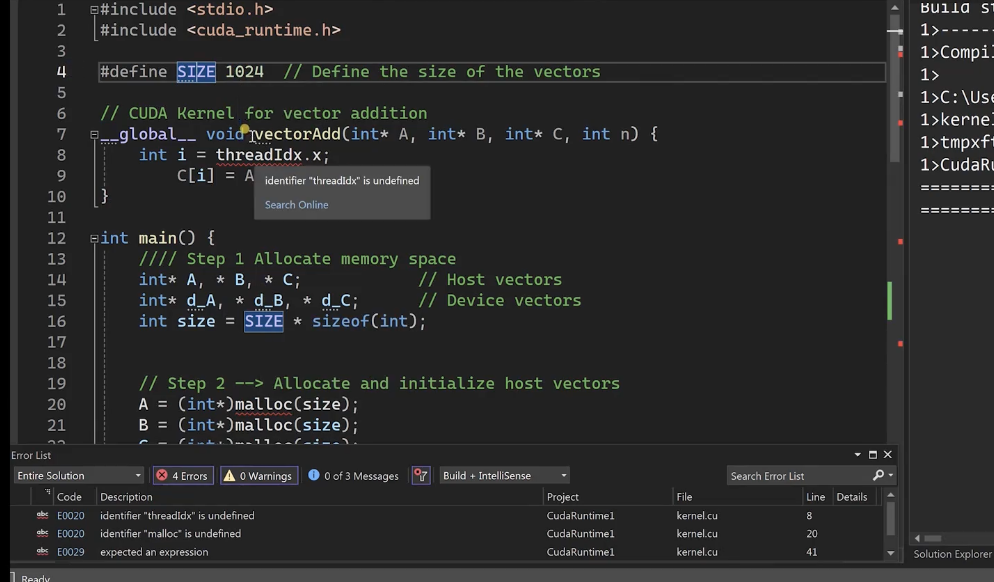
\includegraphics[width=0.75\linewidth]{resources/cuda-076.png}
    \caption{}
    \label{fig:placeholder}
\end{figure}


第三步涉及将这些初始化的A和B值传输到GPU。因为我们的目标是在GPU上执行加法操作，这一步可以通过这2个API或两条指
令实现。有必要将输入数据移动到GPU的内存中。第一个是复制向量A的数据，第二个用于复制向量B的数据。一旦数据进入GPU内
存，我们就可以调用向量加法内核。这可以通过调用GPU内核来实现。如这里的指令所示，这个内核处理A和B的元素以执行加法操作
，并将结果保存在向量C中。正如我们讨论的那样，这条指令包含三个主要部分：内核名称、内核配置（或块和线程的数量），以及最后
是这个内核的输入参数。这就是实现这一点的指令。


在结果安全存储在GPU内存中之后，下一步是将它们传输回CPU内存。在那里你可以打印它们，或将它们发送到另一个阶段，或发送
到另一个GPU内核进行进一步计算等等。它只是一个内存复制操作，但这次它的配置是从GPU、从设备到主机、从GPU到CPU。
如图所示。这个过程的最后一步是释放之前在CPU和GPU上分配的内存空间。这确保了高效的资源管理，并避免内存泄漏。

\subsection{完整代码解析}

如你所见，我以每个向量的大小开始这段代码，这就是我们项目的代码，大小等于1024个元素。每当我们需要改变应用中向量的大小
时，我们所要做的就是来到这里并更改这个值。这就是为什么我们需要在应用开始时预定义大小。然后我们有GPU内核，我们知道这是
一个GPU内核，而不是CPU函数，因为这里的这个部分\texttt{\_\_global\_\_}，这意味着这一部分或这
个内核或这些指令将在GPU端执行，而不是在CPU端。内核名称是\texttt{vectorAdd}，如你所见，它接受四个
值。如我们所看到的，向量A、向量B这些是输入，向量C这是输出或我们将存储结果的地方。然后我们还有另一个变量N，实际上这个
变量等于大小，它将会是1024。但我今天跳过它，在下一个文章中，我将在另一个文章中解释N变量背后所有的技巧。因为我们需要
在这里使用它，但不是今天。

然后我们有这两条指令，实际上我们可以将它们合并为一条指令。我们需要做的就是复制这部分并放在这里第一条指令。但我不想这样做
，因为我在为你们准备更复杂的应用。这里是读取线程ID，正如我们所说，我们有1024个线程，这个将包含线程ID的值，不同的
线程ID将用于遍历这些向量中的所有元素。这里的线程ID将从0到1023。明白吗？这就是GPU内核，它非常简单。

然后这是主函数的开始。如你所见，第一步是分配一些指针以供使用，下一步是在CPU端和GPU端分配空间。例如这三个向量，如你
所见，将用于在CPU内存上为三个向量分配空间，用于向量A、向量B和向量C。如你所见，我们使用\texttt
{malloc}函数来分配这些空间。但是记住，这是每个向量的大小，如你所见，这个大小将被使用。不要忘记我们在这里预定义
了大小，而这个大小并不正好是1024，因为我们乘以了整数值的大小（\texttt{sizeof(int)}）， 这就是我
们使用\texttt{malloc} 函数的方式。总之你需要具备非常简单的C语言背景才能理解这里的一切。

然后我们使用这里的另外三个指针来在GPU内存上分配空间，而不是CPU。这里这是针对CPU的对吧？但这三个指令是为在GPU
内存上分配三个向量所需的空间。如你所见，这是第一个向量，从这个部分；第二个向量；第三个向量。它们都使用相同的大小。

下一步是初始化向量A和向量B。我们不会初始化向量C，因为这是我们将要存储结果的地方，我们不需要用任何值初始化它。这里我们
使用一个for循环来遍历向量A和向量B内的所有元素，我们只是存储一些值。这个for循环的结束条件在这里是1024。如你所
见，例如在A中我们存储I的值，I从0到1024。第一个元素将等于0，第二个元素将等于1，最后一个元素将等于1023。以此
类推。如果I等于0，B的值将等于1023。B也是一样，但它的值等于1024减去I值。这非常简单，没什么难的，但无论如何，
我们不需要关注值本身。你可以用任何你想要的值来初始化A和B。

然后一旦我们初始化了A的值和向量B的值，我们需要将这些值从CPU传输到GPU。因为这里的A和B在CPU端，不在GPU端。
如果你记得，A和B是CPU的，\texttt{d\_A}、\texttt{d\_B}是GPU端的。我们需要做的就是使用这
个函数\texttt{cudaMemcpy}，意思是CUDA的内存复制操作。我们将要从主机复制到设备，主机指的是CPU，
设备指的是GPU，这就是这条指令的用法。我们将要从指令A复制到指令\texttt{d\_A}，这是从CPU，这是到GPU
。我们要复制的数据量等于这个大小。向量B也是如此，如你所见，我们将移动数据，大小等于这个值，从CPU到GPU，从变量B到
GPU上的变量\texttt{d\_B}。我们不需要复制向量C，因为向量C将存储结果。

一旦你通过这两个指令或API将数据放入GPU内存，你需要做的就是执行向量加法内核 \texttt{vectorAdd}内
核。我们在这里启动，我们调用 \texttt{vectorAdd}内核，它将执行这里的这两条指令。我们将使用的配置是我们
的一个块，每个块1024个线程。并且我们将发送或说明这个内核将使用向量A、向量B、向量C，如你所见，以及所有这些向量的大
小作为输入。一旦你调用这个函数，执行将从CPU端转移到GPU端。它会来到这里并执行所有线程，这意味着对所有元素执行加法操
作，并将结果存储在C中。

一旦我们在C中有了结果，这一步之后，我们需要做的就是将数据从GPU内存复制回CPU内存。如你所见，我们将结果复制回主机，
只是为了将这部分与这部分进行比较。\texttt{cudaMemcpyDeviceToHost}，这里我们
有\texttt{HostToDevice}。如你所见，我们要传输或移动的数据量等于这个大小，并且我们从GPU向量移动到
CP U向量 。我需要你注意这里的顺序，这里从GPU到CPU。

一旦我们在向量C上有了数据，而向量C在CPU端，我们就可以打印结果C值。我在这里使用for循环遍历所有元素并打印A、B和
C值。如你所见，A加B等于C。一旦你打印完结果，你需要释放两端所有分配的空间，CPU端和GPU端。如你所见，这里我使
用\texttt{cudaFree} 释放GPU的内存，CPU端也是一样，但只使用一个叫 \texttt{free}的函
数。 正如我告诉你的，它们非常相似，这里的 \texttt{free}，这里的\texttt{cudaFree}。但是因
为这将释放GPU上的空间，我们在这里使用了CUDA术语。

如你所见，这些是主要步骤。我们需要做的就是来到这里并构建，以确保没有任何错误。看这里，这个部分我从下面移到了右边。如你所
见，我们的应用编译正确。如你所见，构建成功，所以我们没有任何失败。我们现在需要做的就是运行这个应用。如你所见，我们正在打
印值，因为所有操作都已经执行完毕了。这些值来自这个部分，来自这个for循环，明白吗？这意味着之前所有的步骤都已正确执行。
是的，这些就是结果。为了让它更简单，就在这里用比如32个值，然后编译并运行。让我们放大看看这些值。这是第一个值，A的第一
个元素加上B的第一个元素，这就是结果。如果你还记得这里的初始化过程，这个部分我们用相同的值从0到32或31初始化了A向量
，而B向量一开始以32结束。这些是A的值，从零开始到31结束。这就是初始化过程，你可以选择任何其他值，看看它们是否正确。
我们的结果给出了正确的值。例如，23加9等于32。

我们现在需要做的就是改变块和线程的数量。但我要在这个文章中跳过它，在另一个文章中再做，因为我不想让这个文章太长。请跟进本
课程的所有文章，以便能够理解一切。今天就到这里，下个文章见。
